\chapter{Forward Model}
\label{ch:formodel}

In this chapter, we present the forward model on which we apply all our methodology. We follow the Michelson Interferometer for Passive Atmospheric Sounding (MIPAS) handbook \cite{mipas2000handbook} and simulate data according to a cloud-free atmosphere in local thermodynamic equilibrium and assume a measurement instrument with infinite spectral resolution and no pointing errors.
We do not include any other instrument specific details, such as sensor area or antenna response, as they are not available to us. 
\begin{figure}[ht!]
	\centering
	\input{LIMB.pdf_tex}
	\caption[Schematic of measurement and analysis geometry.]{Schematic of measurement and analysis geometry, not to scale.
		The stationary satellite, at a constant height $h_\text{sat}$ above Earth, takes $m = 30$ measurements along its line-of-sight defined by the line $\Gamma_j$.
		Each measurement has a limb height $\ell_j$, $j=1,2,\dots,m$ defined as the closest distance of $\Gamma_j$ to the Earth's surface.
		Between $h_{L,0} \approx 7$km and $h_{L,n} \approx 82$km, the stratosphere is discretised into $n =34$ layers as illustrated by the solid green lines.}
	\label{fig:LIMB}
\end{figure}


A satellite at a constant height $h_{\text{sat}}$ points through the atmosphere (limb-sounding) and measures thermal radiation of gas molecules along its straight line of sight $\Gamma_j$, see  Figure~\ref{fig:LIMB}.
One measurement of the thermal radiation of one specific molecule, in our case ozone, denoted by the ozone volume mixing ratio (VMR) $x(r)$ at distance $r$ from the satellite, at the wave number $\nu$, is given by the path integral
\begin{align}
	\label{eq:RTE} 
	y_j =   \int_{\Gamma_j}  B(\nu,T) k(\nu, T)   \frac{p(T)}{k_{\text{B}} T(r)}  x(r)  \tau(r) \text{d}r + \eta_j \, \\
	\tau(r) = \exp{ \Bigl\{ - \int^{r}_{r_\text{obs}}  k(\nu, T)   \frac{p(T)}{k_B T(r^{\prime})}  x(r^{\prime}) \text{d}r^{\prime} \Bigr\} } \, ,\label{eq:absRTE} 
\end{align}
which is the radiative transfer equation (RTE)~\cite{mipas2000handbook}.
For more information on the processes within the atmosphere for ozone, we refer to \cite{Lee2020NightOzone}.
We define a tangent height $h_{\ell_j}$ and $\Gamma_j$ for each $j=1,2,\ldots,m$, so that the data vector $\bm{y} \in \mathbb{R}^m$ including some noise $\eta_j$.
Within the atmosphere, the number density $p(T) / (k_{\text{B}} T(r))$ of molecules is dependent on the pressure $p(T)$, the temperature $T(r)$, and the Boltzmann constant $k_{\text{B}}$.
The factor $\tau(r)\leq 1$ accounts for re-absorption of the radiation along the line-of-sight, which makes the RTE non-linear.
The absorption constant
\begin{align}
	k(\nu, T) = L(\nu, T_{\text{ref}}) \frac{Q(T_{\text{ref}})}{Q(T)} \frac{ \exp{\{ - c_2 E^{\prime \prime} / T\}} }{\exp{\{ - c_2 E^{\prime \prime} / T_{\text{ref}} \}}} \frac{ 1- \exp{\{ - c_2 \nu  / T \}} }{1 - \exp{\{ - c_2 \nu / T_{\text{ref}} \}}}
\end{align}
is dependent on the line intensity $L(\nu, T_{\text{ref}})$ at reference temperature $T_{\text{ref}} =296K $, the lower-state energy of the transition $ E^{\prime \prime} $, the second radiation constant $c2=1.4387769\text{cmK}$ all provided by the HITRAN database \cite{gordon2022hitran2020}.
Since we assume that the measurement device has negligible frequency window we neglect line broadening around $\nu_0$ for the calculations of $L(\nu, T_{\text{ref}})$, which would normally be modelled as a convolution of the normalised Lorentz profile (collisional/pressure broadening) and the normalised Doppler (thermal broadening) profile \cite{mipas2000handbook}.
Additionally, since we target one specific molecule, we simplify the calculation of $k(\nu, T)$, which usually involves summing the individual absorption constants for each targeted molecule weighted by the respective volume mixing ratio \cite{mipas2000handbook}.
The total internal partition function for the lower-state energy is given as:
\begin{align}
	Q(T )= g^{\prime \prime} \exp{\{ - \frac{ c_2 E^{\prime \prime} }{T}\}} \, ,
\end{align}
with the statistical weight $ g^{\prime \prime}$ (also called the degeneracy factor) accounting for the molecule's non-rotational and rotational energy states, see \cite{vsimevckova2006einstein}.
Under the assumption of local thermodynamic equilibrium (LTE), the black body radiation acts as a source function
\begin{align}
	B(\nu,T)   = \frac{2 h c^2 \nu^3}{\exp{\{\frac{hc\nu}{k_B T}\}}-1}\, ,
\end{align}
with Planck's constant $h$ and speed of light $c$.
For fundamentals on the Radiative transfer equation we recommend \cite[Chapter 1]{rybicki2000rte}, and for a more comprehensive model we refer to \cite{read2006forwardModel}

To enable matrix-vector multiplication, we discretise the atmosphere in $n$ layers, where the $i^\text{th}$ layer is defined by two spheres of radii $h_{L,i-1} < h_{L,i}$, for $i = 1, \dots, n$, with $h_{L,0}$ and $h_{L,n} $.
Then we can discretise the ozone, pressure and temperature profiles as a function of height; in between the heights $h_{L,i-1}$ and $h_{L,i}$, each of the ozone concentration $x_{i}$, the pressure $p_{i}$, the temperature $T_{i}$, as well as all other height dependent parameters are assumed to be constant.
Above $h_{L, n}$ and below $h_{L,0} $, the ozone concentration is set to zero, so no signal can be obtained.
Depending on the parameter of interest, which is either the ozone volume mixing ratio $\bm{x} =\{x_1,x_2,\ldots,x_n\} \in \mathbb{R}^{n}$ or the fraction of pressure and temperature $\bm{p/T}= \{p_1/T_1,p_2/T_2,\ldots,p_n/T_n\} \in \mathbb{R}^{n} $
we rewrite the integral in Eq.~\eqref{eq:RTE} for one noise free measurement, using the trapezoidal rule, as a vector-vector multiplication $\bm{A_{j}}(\bm{x},  \bm{p},\bm{T}) \, \bm{x} $ or $\bm{A_{j}}(\bm{x},  \bm{p},\bm{T}) \, \bm{p}/ \bm{T} $, where the non-linear absorption $\tau(r)$ is included in $\bm{A_{j}}(\bm{x},  \bm{p},\bm{T}) \in \mathbb{R}^{n}$ which is the $j$-th row of the matrix $\bm{A}(\bm{x},  \bm{p},\bm{T})$.
Then given a noise vector $\bm{\eta} \in \mathbb{R}^{m}$ the data vector
\begin{align}
	\bm{y} = \bm{A}_{NL} \, \bm{x} + \bm{\eta}= \bm{A}_{NL} \,
	\frac{ \bm{p}}{\bm{T}} + \bm{\eta} \, 
\end{align}
is based on a matrix-vector multiplication.
Here we define the non-linear forward model matrix as $\bm{A}_{NL} \coloneqq \bm{A}(\bm{x},  \bm{p},\bm{T})   \in \mathbb{R}^{m \times n}$ for simplicity, so that $\bm{A}_{NL}\bm{x}$ or $\bm{A}_{NL}\bm{p}/\bm{T}$ implies the construction of $\bm{A}_{NL}$ and similarly for $\bm{A}_L$, which denotes the linear forward model matrix and neglects abortion (e.g. set $\tau = 1$ in Eq.~\eqref{eq:absRTE}).
Further, we classify the inverse problem as weakly non-linear, see e.g. Fig. \ref{fig:MapAsses}, as neglecting the absorption changes the measurements only slightly.



\section{Singular Value Decomposition of the Forward Model}
\label{sec:SVD}
Before simulating some data, we provide a quick and intuitive way of assessing if the data collection is effective, how much information is passed through the forward model, depending on how we measure and how the signal-to-noise ratio affects that information.
One way of doing this is via a singular value decomposition (SVD) of the forward model matrix
\begin{align}
	\bm{A} = \sum_{i =1}^{r} \bm{u}_i  \sigma_i \bm{v}^T_i = \bm{U} \bm{\Sigma} \bm{V}^T
\end{align}
where $r = \min\{m,n\}$ for a forward model $\bm{A} \in \mathbb{R}^{m \times n}$.
Consider noise free measurements $\bm{A}\bm{x}$ for a satellite at a fixed height of $h_{\text{sat}} = 500$km above sea level, where $\bm{x}$ is the ozone VMR, then the SVD gives us information on how information is picked up from the parameter space by the forward model, described through the right singular values $\bm{v}_i$.
The singular values $\sigma_i $, ordered in size from the largest $\sigma_1$ to the smallest $\sigma_{r}$, weight that information from the right singular values to the left singular values $\bm{u}_i$, which project onto the data space.
If we have lots of high-valued singular values, we can say that the forward model is informative and vice versa.
The right singular vectors indicate which structures of the parameter space are picked up by the model.

Further, for very small singular values $\sigma_i \ll \sigma_1/\text{SNR}$ below the RMS noise level or the noise standard deviation (STD), we can introduce an effective rank $r_{\text{eff}} \leq r$.
Then information of parameter space spanned by $ \{\bm{v}_{r_{\text{eff}} +1}, \dots ,\bm{v}_r \}$ is not passed through the forward model and the data is noise dominated in the corresponding data space, see Figure \ref{fig:nullSpace}.
This is based on the rough assumption that if we define the signal-to-noise ratio (SNR) as
\begin{align}
	\text{SNR} \coloneqq \frac{\max(y)}{\text{STD noise}} = \frac{\text{peak signal}}{\text{RMS noise}} \text{\cite{fox2025BlokkLecNot}} \label{eq:SNR}
\end{align}
then the maximum singular value $\max(y) \approx \sigma_1$ and the information transmitted through the forward model corresponds roughly to the singular values $\sigma_i \gtrsim \max(y)/ \text{SNR}$.
See \cite{tan2016LecNot} for a more comprehensive analysis.

\begin{figure}[ht!]
	\centering
	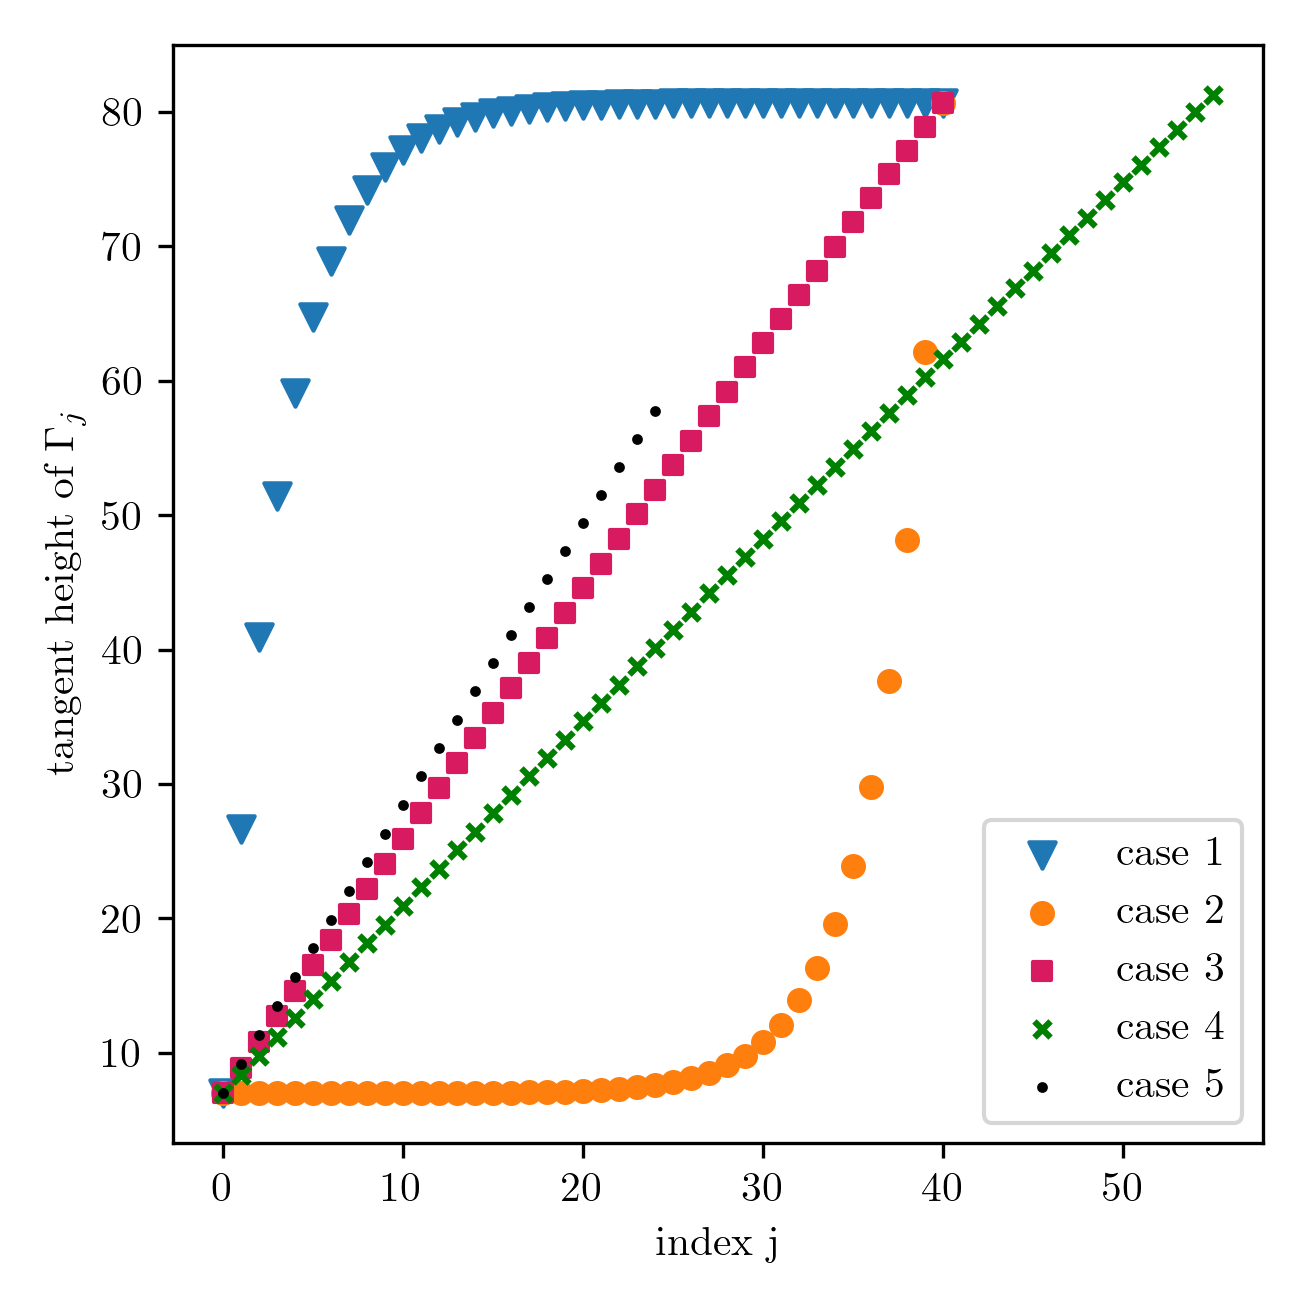
\includegraphics{MeasTangHeight.png}
	\caption[Tangent heights for different sequences of measurements.]{We plot the tangent heights for different cases of measurements.}
	\label{fig:TangHCases}
\end{figure}
\begin{figure}[ht!]
	\centering
	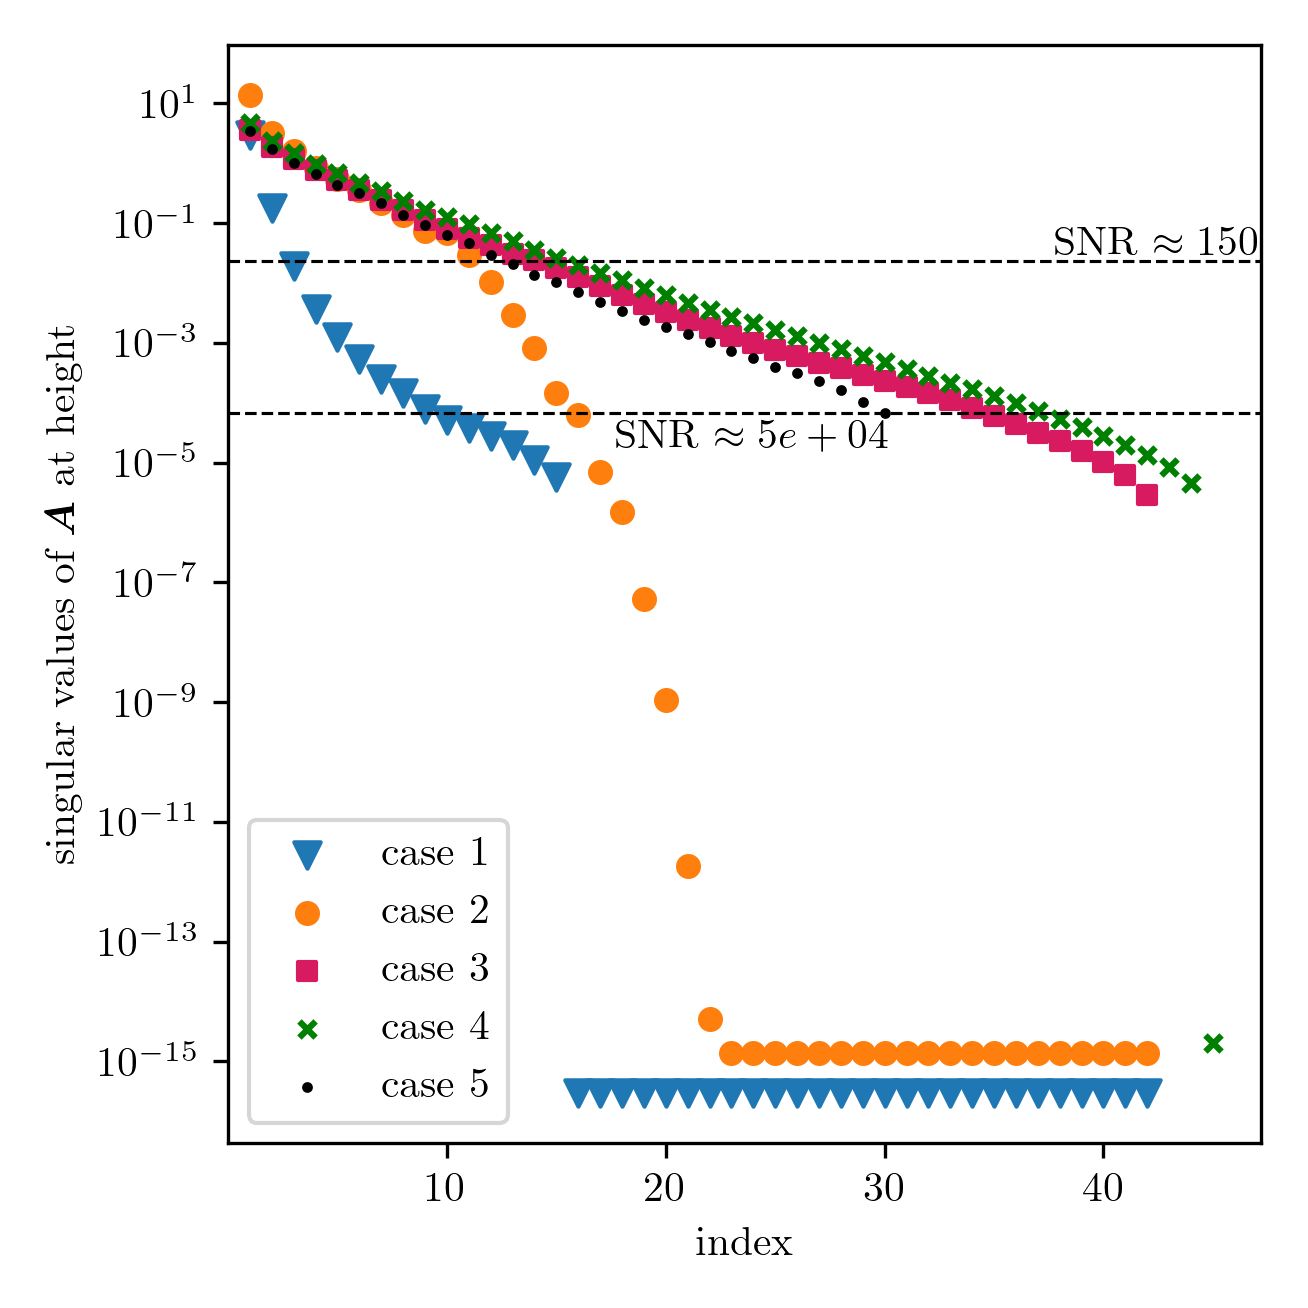
\includegraphics{SingValA.png}
	\caption[Singular values of linear forward model matrix for different sequences of measurements.]{We plot the singular values of the forward model matrix for different sequences of measurements.
		The corresponding tangent heights of the test cases are plotted in Fig. \ref{fig:TangHCases}. The dotted vertical line marks where the singular values are dominated by noise according to a SNR.}
	\label{fig:SingA}
\end{figure}
Next, we plot the singular values for 5 different measurement scenarios, where we either measure at equidistance spaced tangent heights or collect more data from high signal regions at low altitudes, to see which of the tested cases is most effective.
We assess the number of singular values above and below a certain SNR visually.
Our objective is to measure ozone $\bm{x}$ so our forward model $\bm{A}$ includes temperature and pressure, the latter is dominant, see Fig. \ref{fig:PriorPressOverTemp}, and decreases exponentially in height and hence does affect the information passed through the model.
If the pressure is high, the noise is low, and if the pressure is low, the data is noise-dominated.
We start with case 3 in Fig. \ref{fig:TangHCases} where measurements are spaced according to a pointing accuracy of $150\text{arc sec}$, given to us by the team of the University of New South Wales Canberra Space \cite{CubeSatInternal}.
The pointing accuracy determines how well the satellite can point in a certain direction and, hence, roughly the spacing in between two measurements.
The corresponding singular values are plotted in Fig. \ref{fig:SingA}, of which the first 25 decrease linearly in log-space and about 10-15 singular values lie above the SNR.
In comparison, if we measure a lot of times in regions where the data is noise-dominated (high altitude), case 1, we do obtain more information since the singular values decrease rapidly.
Measuring lots of times at low altitudes, where the data is informative, and less at higher altitudes, case 2, does not seem optimal either, as we observe one larger singular value, but the other singular values decrease faster compared to case 3.
Now, if we double the number of measurements compared to case 3, see case 4, we do get slightly larger singular values, but not significantly so that it would be worth the engineering effort required to achieve that.
The measurements with equidistance-spaced tangent height seem to be most informative.
By exploratory analysis, we find that we can tolerate a slightly larger distance between tangent heights (pointing accuracy of $175\text{arc sec}$) than required by \cite{CubeSatInternal}, see case 5.
In that case, we also stop measuring when the signal is too noisy and decrease the number of measurements taken without losing information.
We note that if one wanted to obtain all information provided by the forward model, we would need a signal-to-noise ratio of roughly $10^7$.

In principle, we show that it does not depend on how one measures, one can not get more information by measuring more in regions where the information content is low or high.
This contradicts the current measurement setup on the AURA MLS  \cite{livesey2006retrieval}, which reports high noise in lower atmospheric regions, due to thermal radiation from the earth, and measures more in those regions.


\begin{figure}[ht!]
	\centering
	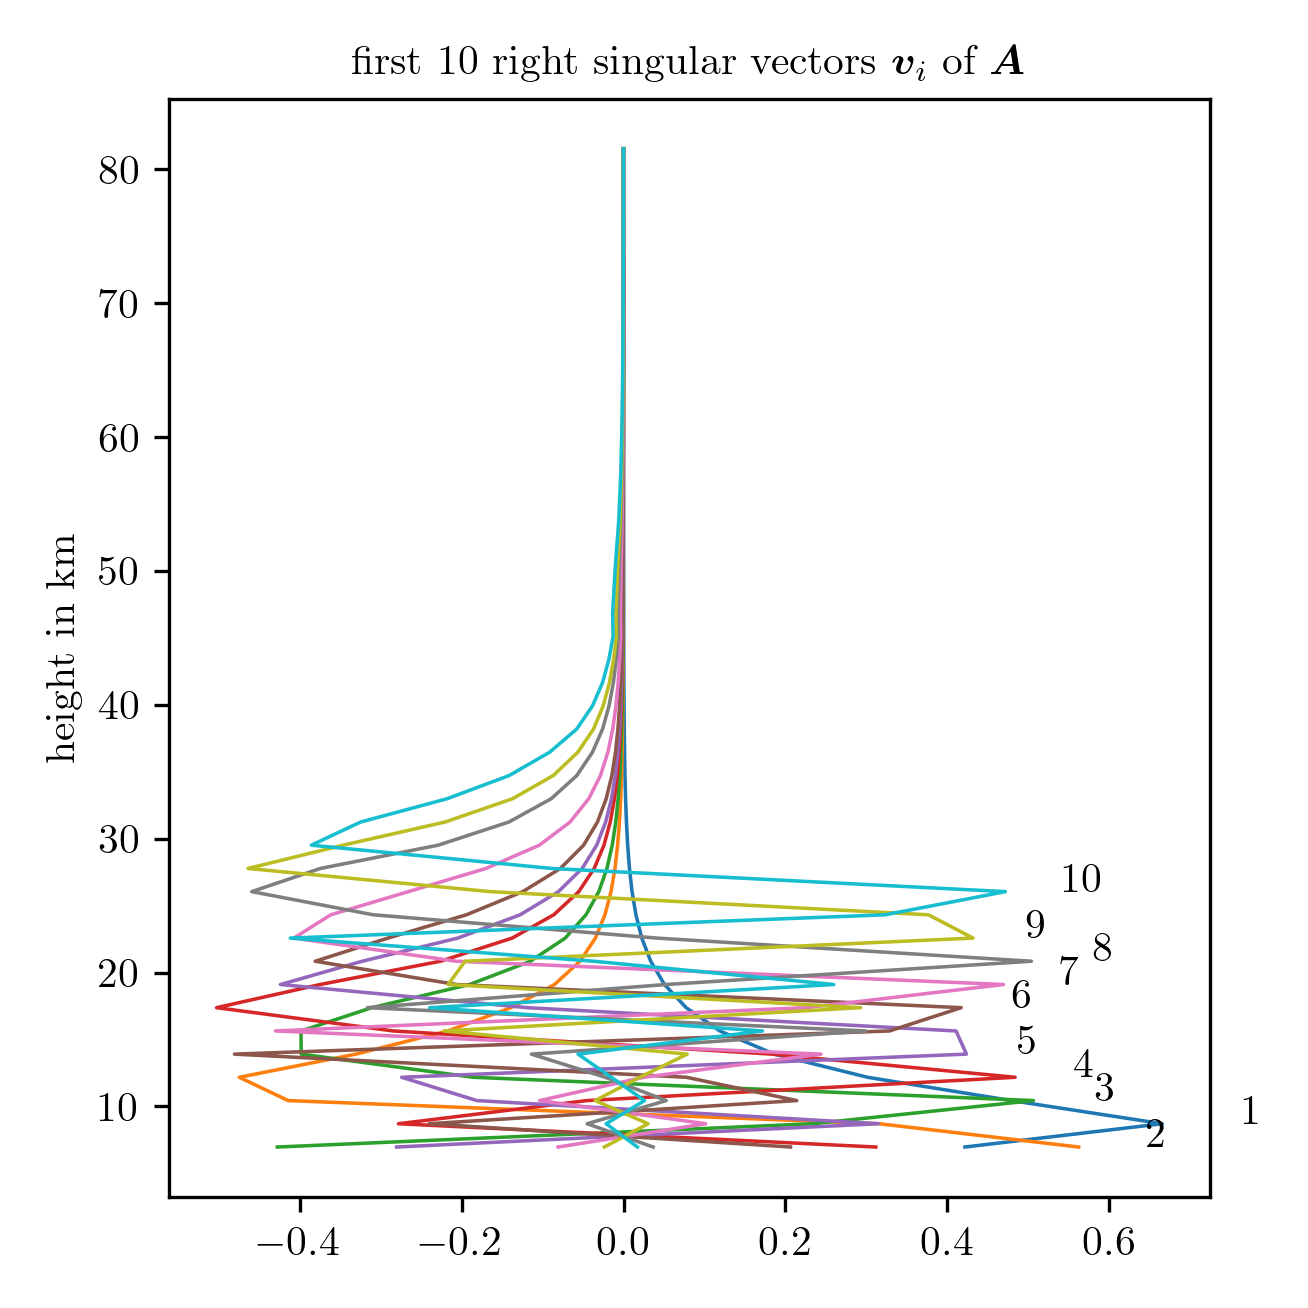
\includegraphics{SingVecA.png}
	\caption[First 10 right singular vectors of forward model.]{We plot the first 10 right singular vectors of the forward model matrix for case 5 sequence of measurements, see Fig. \ref{fig:SingA}. These singular vectors correspond to high singular values of the forward model, see Fig. \ref{fig:SingA}.}
	\label{fig:SingVecA}
\end{figure}
\begin{figure}[ht!]
	\centering
	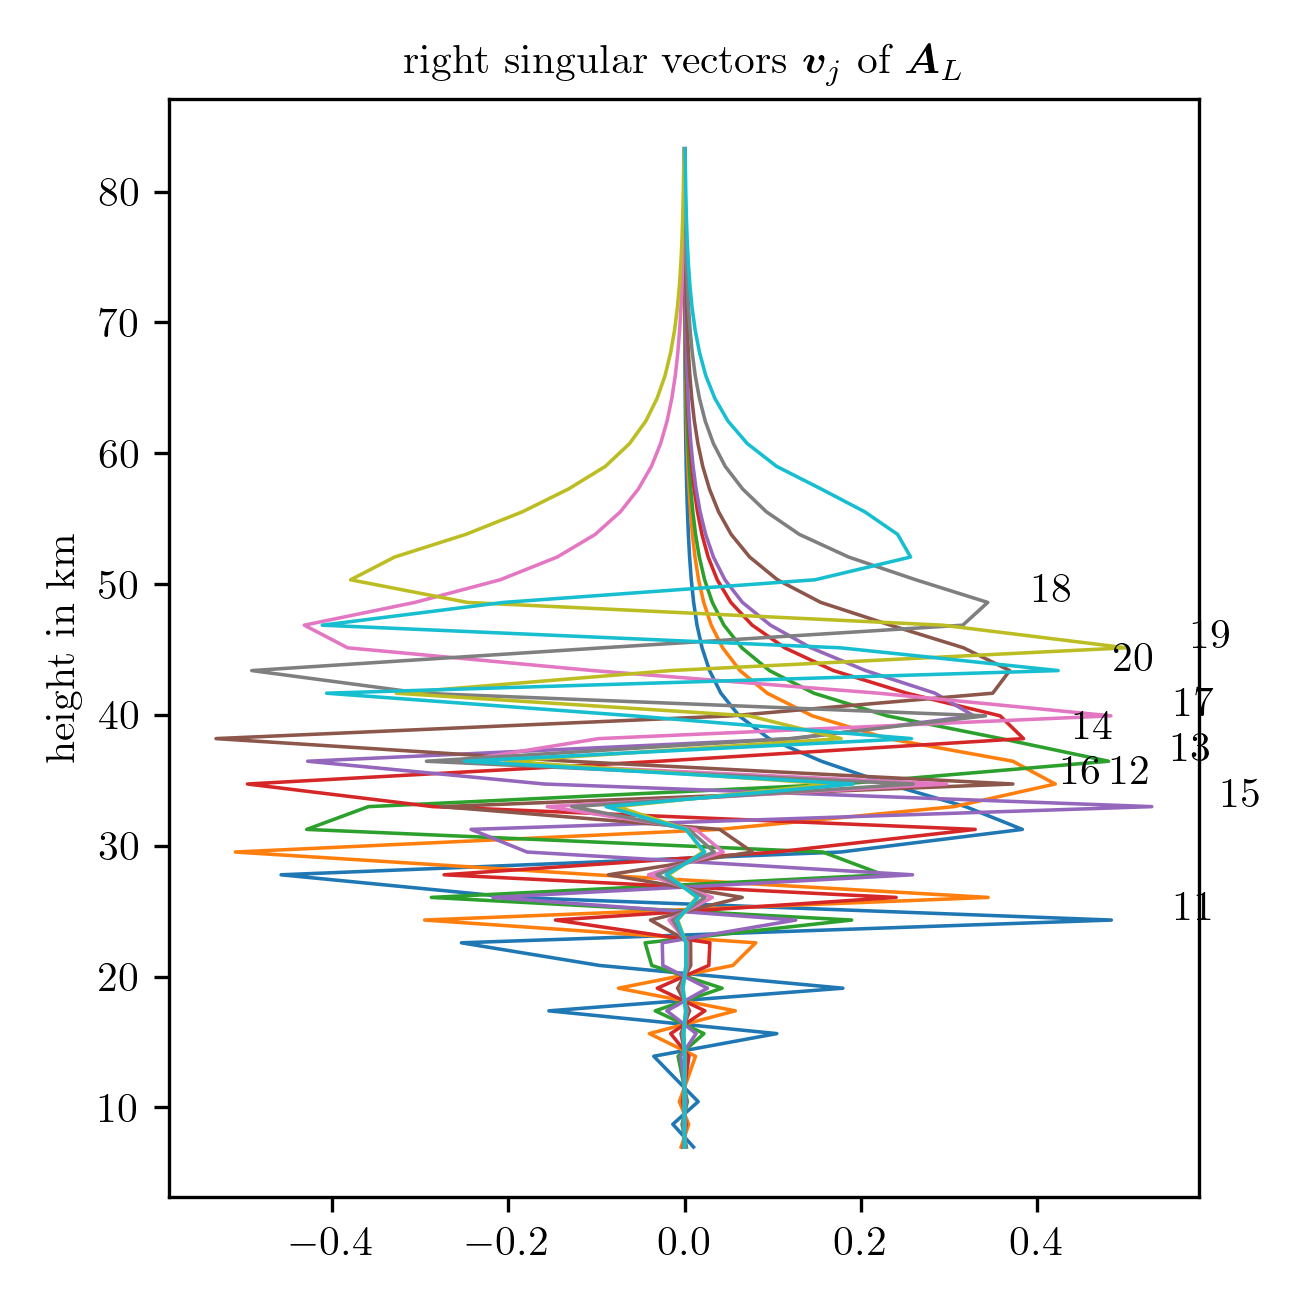
\includegraphics{MiddleVecA.png}
	\caption[Right singular vectors 11 to 19 of forward model.]{We plot the right singular vectors with index $i = 11,\dots, 19$ of the forward model matrix for case 5 sequence of measurements, see Fig. \ref{fig:SingA}.
		These singular vectors correspond to singular values around the noise level of the measurement, see Fig. \ref{fig:SingA}.}
	\label{fig:middleSpace}
\end{figure}
\begin{figure}[ht!]
	\centering
	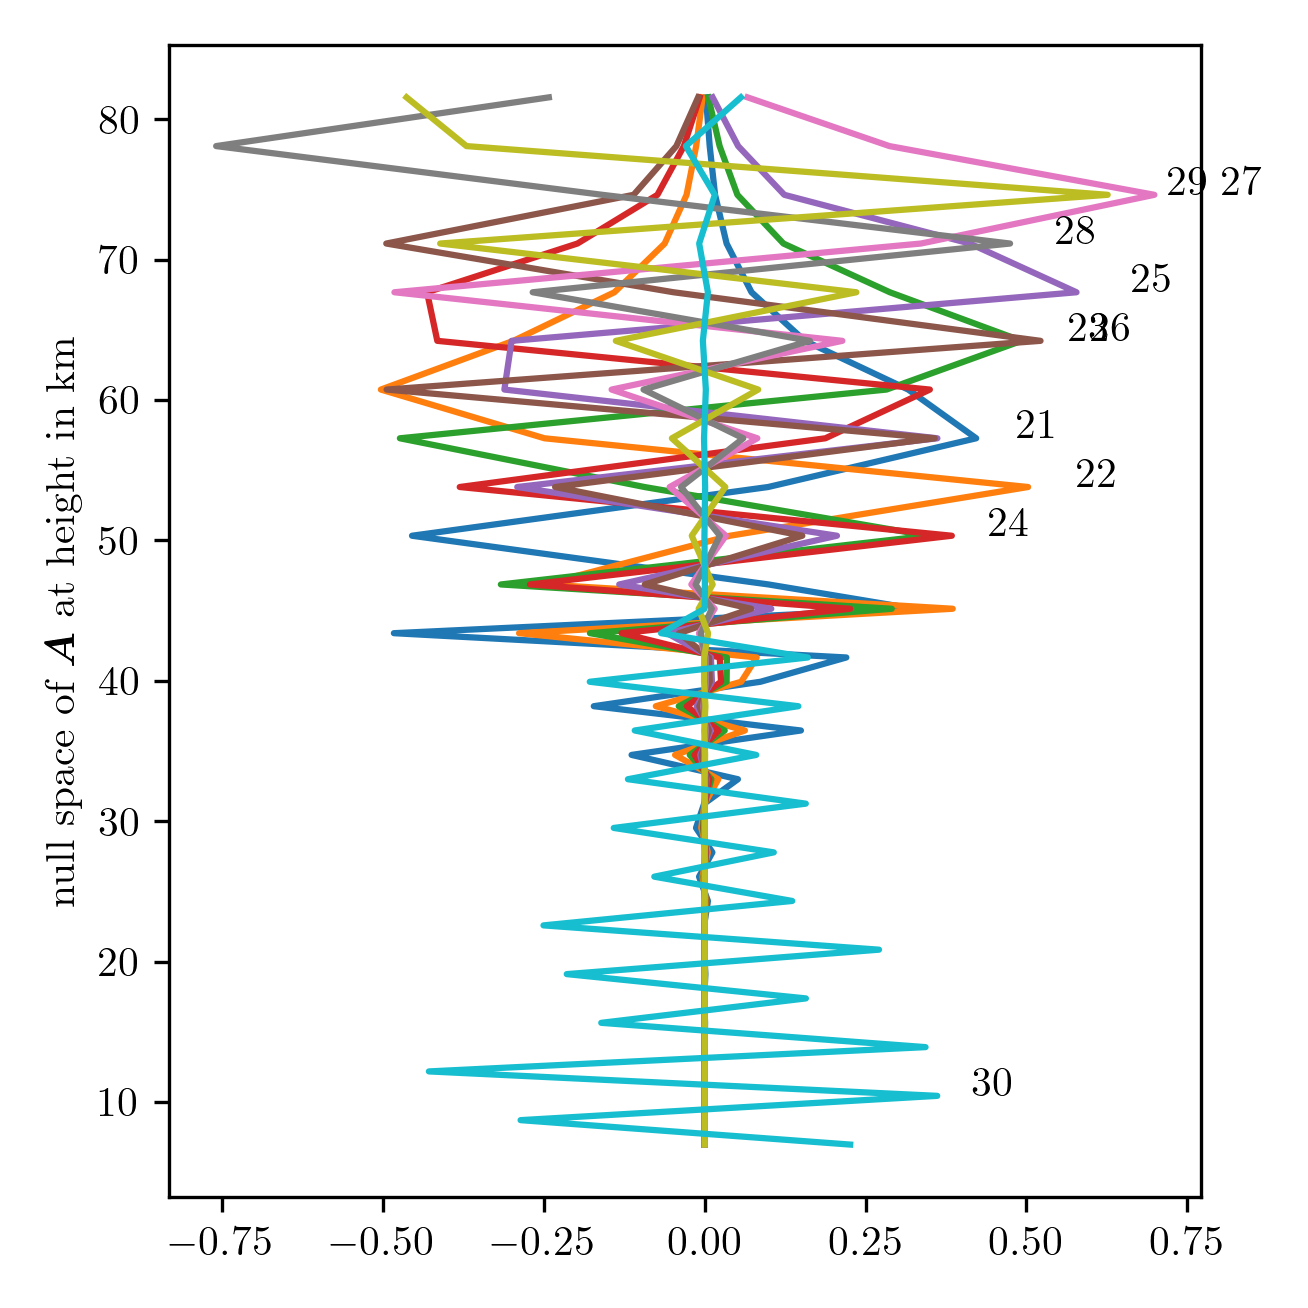
\includegraphics{NullVecA.png}
	\caption[Last 5 right singular vectors of forward model.]{We plot the last 5 right singular vectors of the forward model matrix for the case 5 sequence of measurements, as displayed in Fig. \ref{fig:TangHCases}. These singular vectors correspond to small singular values of the forward model, see Fig. \ref{fig:SingA}.}
	\label{fig:nullSpace}
\end{figure}

Consequently, we proceed with case 5 and plot the right singular vectors of the forward model versus height in the atmosphere to see where our model is most informative, or which structures of the parameter space are picked up by the model.
The first 10 right singular vectors, in Fig. \ref{fig:SingVecA}, corresponding to the 10 largest singular values, pick up structures in lower atmospheric regions.
So we can assume that, given some data, we will be able to provide good reconstructions of the parameter in lower altitudes.
Next, we plot the right singular vectors corresponding to the singular values $\sigma_j$ for $j = 11, \dots, 20$ in Fig. \ref{fig:middleSpace}, where the nose starts to dominate the data.
These singular values lie in regions around the SNR, see Fig. \ref{fig:SingA}, and pick up values in the middle of the atmosphere.
Consequently, we expect a higher uncertainty of reconstructed parameter values in the middle atmospheric regions.
The singular vectors corresponding to the last 5 singular values pick up structures in higher altitudes, but since the singular values are very small, we will not be able to retrieve those structures.
More specifically, the retrieved parameter values at higher altitudes will be fully determined by the prior or, in the case of regularisation, by the regulariser \cite{tan2016LecNot}.

